% Chapter Template

\chapter{Theoretical Background} % Main chapter title

\label{Chapter2} % Change X to a consecutive number; for referencing this chapter elsewhere, use \ref{ChapterX}

\lhead{Chapter 2. \emph{Theoretical Background}}
This chapter is devoted to present the theoretical foundations and formalism of Density Functional Theory (DFT) and related methods required for the development of the results presented in this work. Starting with the many-body Schrödinger equation, this chapter covers the Born-Oppenheimer approximation, the Hartree-Fock approximation, Hohenberg-Kohn theorems, the Kohn-Sham equations, exchange-correlation functionals, and definitions on Ab initio molecular dynamics (AIMD) and machine learning force fields (MLFFs), along with implementation details in the Vienna Ab initio Simulation Package (VASP).

Ultimately, this chapter aims to provide a comprehensive understanding of the theoretical framework that underpins the computational methods utilised in this work, enabling the reader to grasp the principles and assumptions that govern the simulations and analyses performed throughout.

\section{Many Body Schrödinger Equation}
In our efforts to unravel the tapestry of materials, quantum mechanics lights our path towards describing the complex, yet fundamental interactions that govern particle behaviour at the atomic scale. Our journey shall commence by describing the physical laws that shape the interactions among particles constituting a system---electrons and nuclei alike. 

\subsection{The Coulomb Interaction}

Materials may be thought of as complex assemblies of electrons and nuclei, held together by a delicate balance between attractive Coulomb interactions---primarily between electrons and nuclei---and repulsive interactions between like-charged particles, such as electron-electron and nucleus-nucleus pairs, which govern the overall dynamics of the material system\supercite{giustino2014materials, sholl2023density, kaxiras2003atomic}.  From classical electrostatics, these interactions can be mathematically expressed as follows: 

\begin{itemize}
\item Electron-electron interactions 
  \begin{equation}
    \label{eq1}
    \hat{V}_{ee} = \frac{1}{2} \sum_{i\neq j} \frac{e^2}{4\pi\epsilon_0 |\mathbf{r}_i - \mathbf{r}_j|}
  \end{equation}
\item Electron-nucleus interactions 
  \begin{equation}
    \label{eq2}
    \hat{V}_{nn} = \frac{1}{2} \sum_{I\neq J} \frac{e^2}{4\pi\epsilon_0} \frac{Z_I Z_J}{|\mathbf{R}_I - \mathbf{R}_J|}
  \end{equation}
\item Electron-nuclei interactions 
\begin{equation}
    \label{eq3}
    \hat{V}_{en} = -\sum_{i\neq I} \frac{e^2}{4\pi\epsilon_0} \frac{Z_I}{|\mathbf{r}_i - \mathbf{R}_I|}
  \end{equation}
\end{itemize}

where $e$ is the electronic charge, $\epsilon_0$ is the vacuum permittivity, $Z_I$ and $Z_J$ are the atomic numbers of nuclei $I$ and $J$, respectively, and $\mathbf{r}_i$ and $\mathbf{R}_I$ are the position vectors of electrons and nuclei, respectively. Moreover, we must also consider the kinetic energy of the collection of electrons and nuclei
\begin{equation}
    \label{eq4}
    \hat{T} = -\sum_i \frac{\hbar^2}{2m_e} \nabla_i^2 - \sum_I \frac{\hbar^2}{2M_I} \nabla_I^2
\end{equation}
where $\hbar$ is the reduced Planck's constant, $m_e$ is the electron mass, and $M_I$ is the mass of the nucleus $I$.

\subsection{The Time-Independent Schrödinger Equation}
The Time-Independent Schrödinger Equation (TISE) lies at the heart of non-relativistic quantum mechanics, providing a mathematical framework to describe stationary electronic states of quantum systems. It takes the following form:
\begin{equation}
  \label{eq5}
  \hat{H} \psi(\mathbf{r}) = E \psi(\mathbf{r})
\end{equation}
where $\hat{H}$ is the Hamiltonian of the system, incorporating both the kinetic and potential energies, $\psi(\mathbf{r})$ is an eigenstate of the system, and $E$ is the energy eigenvalue associated with eigenstate $\psi(\mathbf{r})$.  It is important to note that Equation \ref{eq5} is only applicable to a single particle, yet a material system is composed of many electrons ($N$) and nuclei ($M$) with spatial coordinates $\mathbf{r}_1, \mathbf{r}_2, \ldots, \mathbf{r}_N$ and $\mathbf{R}_1, \mathbf{R}_2, \ldots, \mathbf{R}_M$, respectively. Therefore, we must introduce a so-called many-body wavefunction given by:
\begin{equation}
  \Psi(\mathbf{r}_1, \mathbf{r}_2, \ldots, \mathbf{r}_N, \mathbf{R}_1, \mathbf{R}_2, \ldots, \mathbf{R}_M)
  \label{eq5b}
\end{equation}
On this basis, the many-body version of Equation \ref{eq5} shall be constructed by combining the kinetic (Equation \ref{eq4}) and potential (Equations \ref{eq1}, \ref{eq2}, and \ref{eq3}) energy contributions, leading to the following expression:
\begin{equation}
  \label{eq6}
  \begin{split}
    \left[
      -\sum_i \frac{\hbar^2}{2m_e} \nabla_i^2 
      - \sum_I \frac{\hbar^2}{2M_I} \nabla_I^2 
      + \frac{1}{2} \sum_{i\neq j} \frac{e^2}{4\pi\epsilon_0 |\mathbf{r}_i - \mathbf{r}_j|} +\right. \\
      \left. \frac{1}{2} \sum_{I\neq J} \frac{e^2}{4\pi\epsilon_0} \frac{Z_I Z_J}{|\mathbf{R}_I - \mathbf{R}_J|} 
      - \sum_{i, I} \frac{e^2}{4\pi\epsilon_0} \frac{Z_I}{|\mathbf{r}_i - \mathbf{R}_I|}
    \right]\Psi = E_{\text{tot}} \Psi
  \end{split}
\end{equation}
Equation \ref{eq6} provides a complete description of the stationary states of a non-relativistic many-body system, under time-independent conditions and in the absence of external fields. Additionally, we can achieve a more compact formulation by introducing the concept of atomic units. To this end, let us consider the simplest electron-nucleus system---the hydrogen atom---where the electron orbital has an average radius $a_0 \approx 0.529 \, \text{Å}$. Thereby, the Coulomb energy for such a system is given by:
\begin{equation}
  \label{eq7}
  E_{\text{Ha}} = \frac{e^2}{4 \pi \epsilon_0 a_0}
\end{equation}
where 'Ha' stands for Hartree. Within this framework, the Hartree energy represents the Coulomb interaction between two fundamental charges separated by a distance of one Bohr radius ($a_0$). Moreover, the angular momentum quantisation condition for the electron in the hydrogen atom is given by
\begin{equation}
  \label{eq8}
  m_e v a_0 = \hbar
\end{equation}
Additionally, the equilibrium condition between the nuclear attraction and the electron's centrifugal force can be expressed as:
\begin{equation}
  \label{eq9}
  \frac{e^2}{4 \pi \epsilon_0 a_0^2} = \frac{m_e v^2}{a_0}
\end{equation}
By combining Equations \ref{eq7}, \ref{eq8}, and \ref{eq9}, we derive the 
following relationships:
\begin{equation}
  \label{eq10}
  \frac{e^2}{4 \pi \epsilon_0 a_0} = \frac{\hbar^2}{m_e a_0^2}
\end{equation}
\begin{equation}
  \label{eq11}
  \frac{1}{2} m_e v^2 = \frac{1}{2}E_{\text{Ha}}
\end{equation}
This latter relation showcases that the kinetic energy is of the same order as $E_\text{Ha}$, rendering it convenient to normalise Equation \ref{eq6} by this quantity:
\begin{equation}
  \label{eq12}
  \begin{split}
    \left[
      -\sum_i \frac{1}{2}a_0^2 \nabla_i^2 
      - \sum_I \frac{1}{2} \frac{1}{(M_I/m_e)} \nabla_I^2 
      + \frac{1}{2} \sum_{i\neq j} \frac{a_0}{|\mathbf{r}_i - \mathbf{r}_j|}\right. \\
      \left. +  \frac{1}{2} \sum_{I\neq J} Z_I Z_J \frac{a_0}{|\mathbf{R}_I - \mathbf{R}_J|} 
      - \sum_{i, I} Z_I \frac{a_0}{|\mathbf{r}_i - \mathbf{R}_I|}
    \right]\Psi = \frac{E_{\text{tot}}}{E_{\text{Ha}}} \Psi
  \end{split}
\end{equation}
A final simplification involves setting our energy units to Ha, distance units to $a_0$, and mass units to $m_e$. The last missing constant $e$ is set to 1, leading to the following expression: 
\begin{equation}
  \label{eq13}
  \begin{split}
    \left[
      -\sum_i \frac{\nabla_i^2}{2}
      - \sum_I \frac{\nabla_I^2}{2 M_I} 
      + \frac{1}{2} \sum_{i\neq j} \frac{1}{|\mathbf{r}_i - \mathbf{r}_j|} + \right. \\
      \left. \frac{1}{2} \sum_{I\neq J} \frac{Z_I Z_J} {|\mathbf{R}_I - \mathbf{R}_J|} 
      - \sum_{i, I} \frac{Z_I}{|\mathbf{r}_i - \mathbf{R}_I|}
    \right]\Psi = E_{\text{tot}} \Psi
  \end{split}
\end{equation}

Ultimately, even though Equation \ref{eq13} provides an exact method capable of yielding various properties of a material system---such as elastic, thermal, and electronic properties---a combination of mathematical complexity and computational limitations renders it intractable to solve for any realistic system. Moreover, the wavefunction contains vastly more information than is necessary to describe most observable properties of a material. Therefore, we must resort to alternative formulations that allow us to extract only the relevant information from the wavefunction whilst reducing the computational cost of the calculations. The remainder of this chapter is dedicated to presenting such alternative approaches that ultimately lead to the computational methods employed throughout this work.

%-----------------------------------
%	SUBSECTION 1
%-----------------------------------
\section{The Born-Oppenheimer Approximation}
For atoms in a solid, we can think of nuclei as being held immobile in a fixed position, while electrons instantaneously react to any nucleus's movement. This assumption is based on the fact that nuclei are much heavier than electrons---by three to four orders of magnitude---making the former behave like classical particles. Thereby, we can rewrite the many-body wavefunction as a product of two wavefunctions:
\begin{equation}
  \Psi(\mathbf{r}_1, \mathbf{r}_2, \ldots, \mathbf{r}_N, \mathbf{R}_1, \mathbf{R}_2, \ldots, \mathbf{R}_M) = \psi_{\mathbf{R}}(\mathbf{r}_1, \mathbf{r}_2, \ldots, \mathbf{r}_N)\chi(\mathbf{R})
  \label{eq14}
\end{equation}
where $\psi_{\mathbf{R}}$ is the electronic wavefunction parametrised by the nuclear positions $\mathbf{R}$, and $\chi$ is the nuclear wavefunction. Furthermore, this significant mass disparity enables a systematic approximation scheme, wherein the electronic wavefunction is solved for fixed nuclei, and its solution is used as an effective potential for the nuclear dynamics afterwards. First, nuclei' kinetic energy is neglected, as their positions are assumed to be fixed: 
\begin{equation}
  \label{eq15}
  \sum_I \frac{\nabla_I^2}{2 M_I} = 0
  \quad \text{and} \quad  E = E_{\text{tot}} - \sum_{I<J} \frac{Z_I Z_J}{|\mathbf{R}_I - \mathbf{R}_J|}
\end{equation}
Following, we define the Coulomb potential of the nuclei experienced by the electrons as:
\begin{equation}
  \label{eq16}
  V_{\text{n}}(\mathbf{r}) = - \sum_{I} \frac{Z_I}{|\mathbf{r} - \mathbf{R}_I|}
\end{equation}
Then, Equation \ref{eq13} can be rewritten as:
\begin{equation}
  \label{eq17}
  \left[
    -\sum_i \frac{\nabla_i^2}{2} + \sum_i V_{\text{n}}(\mathbf{r}_i) + \frac{1}{2} \sum_{i\neq j} \frac{1}{|\mathbf{r}_i - \mathbf{r}_j|} 
  \right] \Psi = E \Psi 
\end{equation}
Finally, by using Equation \ref{eq14}, we can define the electronic and nuclear Schrödinger equations as follows:
\begin{equation}
  \label{eq18}
  \left[
    -\sum_i \frac{\nabla_i^2}{2} + \sum_i V_{\text{n}}(\mathbf{r}_i) + \frac{1}{2} \sum_{i\neq j} \frac{1}{|\mathbf{r}_i - \mathbf{r}_j|} 
  \right] \psi_{\mathbf{R}} = E_{\mathbf{R}} \psi_{\mathbf{R}}
\end{equation}
\begin{equation}
  \label{eq19}
  \left[
    -\sum_I \frac{\nabla_I^2}{2 M_I} + \sum_{I<J} \frac{Z_I Z_J}{|\mathbf{R}_I - \mathbf{R}_J|} + E(\mathbf{R}_1,\dots,\mathbf{R}_M)\right] \chi(\mathbf{R}) = E_{\text{tot}} \chi(\mathbf{R})
\end{equation}
where $E_{\mathbf{R}}= E(\mathbf{R}_1,\dots,\mathbf{R}_M)$ is the electronic surface energy, which is a function of the nuclear positions, and serves as an effective potential shaping the nuclear dynamics. 

%-----------------------------------
%	SUBSECTION 2
%-----------------------------------

\section{Hartree-Fock Approximation}
The essence of the Hartree-Fock approximation (HFA) is to approximate the interacting many-electron system (Equation \ref{eq17}) by a set of non-interacting single-particle problems subject to an effective mean-field potential\supercite{martin2016interacting, helgaker2014molecular, feng2005introduction}. As a means to this, we first rewrite the total wavefunction for a system with N electrons as the product of single-electron wavefunctions---often referred to as the Hartree approximation\supercite{Hartree1928}---as showcased in Equation \ref{eq20}. 
\begin{equation}
  \Psi^H(\mathbf{r}_1, \dots, \mathbf{r}_N) = \prod_{i=1}^N \phi_i(\mathbf{r}_i)
  \label{eq20}
\end{equation}
Following, we construct the total energy functional as the expectation value of the Hamiltonian operator:
\begin{equation}
  \label{eq21}
\begin{aligned}
  E^{H}[\{\phi_i\}] &= \bigg\langle \Psi^H \bigg| \hat{H} \bigg| \Psi^H \bigg\rangle 
\end{aligned}
\end{equation}
Expanding Equation \ref{eq21}:
\begin{equation}
  \label{eq22}
  \begin{split}
    E^{H}[\{\phi_i\}] &= \sum^N_{i=1} \int \phi_i^*(\mathbf{r}) \left(-\frac{\nabla^2}{2} + V_{\text{n}}(\mathbf{r})\right) \phi_i(\mathbf{r}) d\mathbf{r}  + \frac{1}{2} \sum_{i\neq j} \int\int \frac{|\phi_i(\mathbf{r})|^2 |\phi_j(\mathbf{r'})|^2 }{|\mathbf{r} - \mathbf{r'}|} d\mathbf{r} d\mathbf{r'}
  \end{split}
\end{equation}
where the first term adds up the kinetic energy and electron-nuclear attraction overall electrons, whilst the second accounts for the classical electron-electron repulsion energy averaged over the electron density distribution. In order to find the set of orbitals $\{\phi_i\}$ that minimises the total energy functional, we use the variational principle, where we shall impose the orthonormality condition: 
\begin{equation}
  \label{eq23}
  \int \phi_i^*(\mathbf{r}) \phi_j(\mathbf{r}) d\mathbf{r} = \delta_{ij}
\end{equation}
for what we introduce the Lagrange multipliers $\lambda_{ij}$ to enforce these constraints and define the Lagrangian:
\begin{equation}
  \label{eq24}
  \mathcal{L} = E^H[\{\phi_i\}] - \sum_{i=1}^{N}\lambda_{ij} ( \langle\phi_i|\phi_j\rangle - \delta_{ij})
\end{equation}
which ultimately simplifies to:
\begin{equation}
  \label{eq25}
  \mathcal{L} = E^H[\{\phi_i\}] - \sum_{i=1}^{N}\varepsilon_{i} ( \langle\phi_i|\phi_i\rangle - 1)
\end{equation}

Then, we need to compute the derivative of $\mathcal{L}$ with respect to $\phi_i^*$ and set it to zero:
\begin{equation}
  \label{eq26}
  \frac{\delta \mathcal{L}}{\delta \phi_i^*}(\mathbf{r}) = 0
\end{equation}
which yields the Hartree equation:
\begin{equation}
  \label{eq27}
  \left[-\frac{\nabla^2}{2} + V_{\text{n}}(\mathbf{r}) + V^H_i(\mathbf{r})\right]\phi_i(\mathbf{r})  = \varepsilon_i \phi_i(\mathbf{r})
\end{equation}
where $V_n(\mathbf{r})$ represents the electrostatic interaction between electrons and nuclei, and the Hartree potential 
\begin{equation}
  \label{eq28}
  V^H_i(\mathbf{r}) = \sum_{j\neq i} \int \frac{|\phi_j(\mathbf{r'})|^2}{|\mathbf{r} - \mathbf{r'}|} d\mathbf{r'}
\end{equation}
accounts for the average electrostatic interaction experienced by the $i$-th electron due to all other electrons in the system. This effective mean-field potential replaces the electron-electron interactions, effectively simplifying the many-body problem into single-particle problems. 
\subsection{The Pauli Exclusion Principle}
So far, we have introduced the Hartree approximation, which assumes that the many-electron wavefunction can be expressed as a product of single-particle wavefunctions. However, this approach does not account for the indistinguishability of electrons and the Pauli exclusion principle, which states that no two fermions--- half-spin particles, such as electrons---can reside in the same quantum state simultaneously. In doing so, it imposes a restriction on the possible configurations of electrons in a system that shall be accounted for.
 
 In order to achieve this, V. Fock\supercite{Fock1930} introduced a different approximation to the wavefunction by using a Slater determinant---a mathematical construct that combines one-electron wavefunctions in such a way that satisfies the antisymmetry principle. This is done by expressing the overall wavefunction as the determinant of a matrix of single-electron wavefunctions:
\begin{equation}
  \Psi^{HF}(\mathbf{r}_1, \dots, \mathbf{r}_N) = \frac{1}{\sqrt{N!}} \begin{vmatrix}
    \phi_1(\mathbf{r}_1) & \phi_1(\mathbf{r}_2) & \dots & \phi_1(\mathbf{r}_N)\\
    \phi_2(\mathbf{r}_1) & \phi_2(\mathbf{r}_2) & \dots & \phi_2(\mathbf{r}_N)\\
    \vdots & \vdots & \ddots & \vdots\\
    \phi_N(\mathbf{r}_1) & \phi_N(\mathbf{r}_2) & \dots & \phi_N(\mathbf{r}_N)
  \end{vmatrix}
  \label{eq29}
\end{equation}
where $1/\sqrt{N!}$ is a normalisation factor. To illustrate this, consider a two-electron system with single-particle wavefunctions $\phi_1(\mathbf{r})$ and $\phi_2(\mathbf{r})$. The Slater determinant for this system would be:
\begin{equation}
  \Psi^{HF}(\mathbf{r}_1, \mathbf{r}_2) = \frac{1}{\sqrt{2}} \begin{vmatrix}
    \phi_1(\mathbf{r}_1) & \phi_1(\mathbf{r}_2)\\
    \phi_2(\mathbf{r}_1) & \phi_2(\mathbf{r}_2)
  \end{vmatrix} = \frac{1}{\sqrt{2}} \left[\phi_1(\mathbf{r}_1)\phi_2(\mathbf{r}_2) - \phi_1(\mathbf{r}_2)\phi_2(\mathbf{r}_1))\right]
  \label{eq30}
\end{equation}
Evidently, $\Psi^{HF}(\mathbf{r}_1, \mathbf{r}_2) = -\Psi^{HF}(\mathbf{r}_2, \mathbf{r}_1)$, which satisfies the antisymmetr principle. 
\subsection{The Hartree-Fock Equations}
The Hartree-Fock equations are derived in a similar manner we addressed the Hartree equations. We first define the total energy with the Hartree-Fock wavefunction (Equation \ref{eq29}) 
\begin{equation}
  \label{eq31}
  \begin{split}
    E^{HF}[\{\phi_i\}] &= \bigg\langle \Psi^{HF} \bigg| \hat{H} \bigg| \Psi^{HF} \bigg\rangle\\
    &= \sum_{i} \langle \phi_i \big|\frac{\nabla^2}{2} + V_{\text{n}}(\mathbf{r})\big| \phi_i \rangle\\
    &+ \frac{1}{2} \sum_{i\neq j} \langle \phi_i \phi_j \big| \frac{1}{|\mathbf{r}_i - \mathbf{r}_j|} \big| \phi_i \phi_j\rangle\\
    &- \frac{1}{2} \sum_{i\neq j} \langle \phi_i \phi_j \big| \frac{1}{|\mathbf{r}_i - \mathbf{r}_j|} \big| \phi_j \phi_i\rangle
  \end{split}
\end{equation}
Consequently, using the variational principle, we derive the Hartree-Fock equations: 
\begin{equation}
  \label{eq32}
  \left[-\frac{\nabla^2}{2} + V_{\text{n}}(\mathbf{r}) + V^H_i(\mathbf{r}) +\right]\phi_i(\mathbf{r})
  - \sum_{j\neq i} \langle \phi_j \big| \frac{1}{|\mathbf{r}_i - \mathbf{r}_j|} \big| \phi_i \rangle \phi_j(\mathbf{r})
  = \varepsilon_i \phi_i(\mathbf{r})
\end{equation}
Noticeably, Equation \ref{eq32} has an extra term compared with the Hartree equation (Equation \ref{eq27}). This term is called the "exchange" term\supercite{kaxiras2003atomic}, and describes the effects of exchange between electrons. It is convenient to try to express the Hartree-Fock equations in a more compact form, so we define the single-particle and total densities as 
\begin{equation}
  \label{eq33}
  \rho_i(\mathbf{r}) = |\phi_i(\mathbf{r})|^2
\end{equation}
\begin{equation}
  \label{eq34}
  \rho(\mathbf{r}) = \sum_i \rho_i(\mathbf{r}) 
\end{equation}
so the Hartree potential can be expressed as 
\begin{equation}
  \label{eq35}
  V^H_i(\mathbf{r}) = \sum_{j\neq i}  \int \frac{\rho_j(\mathbf{r'})}{|\mathbf{r} - \mathbf{r'}|} d\mathbf{r'} 
  = \int \frac{\rho(\mathbf{r'}) - \rho_i(\mathbf{r'})}{|\mathbf{r} - \mathbf{r'}|} d\mathbf{r'}
\end{equation}
Therefore, the single-particle exchange density can be constructed as 
\begin{equation}
  \label{eq36}
  \rho^X_i(\mathbf{r}, \mathbf{r'}) = \sum_{j\neq i}\frac{\phi_i(\mathbf{r'})\phi^*_i(\mathbf{r})\phi_j(\mathbf{r})\phi^*_j(\mathbf{r'})}{\phi_i(\mathbf{r})\phi^*_i(\mathbf{r})}
\end{equation}
Finally, the Hartree-Fock equations take the form 
\begin{equation}
  \label{eq37}
  \left[-\frac{\nabla^2}{2} + V_{\text{n}}(\mathbf{r}) + V^H_i(\mathbf{r}) + V^X_i(\mathbf{r})\right]\phi_i(\mathbf{r}) = \varepsilon_i \phi_i(\mathbf{r})
\end{equation}
where $V^X_i$ stands for the exchange potential
\begin{equation}
  \label{eq38}
  V^X_i(\mathbf{r}) = -\int \frac{\rho^X_i(\mathbf{r}, \mathbf{r'})}{|\mathbf{r} - \mathbf{r'}|} d\mathbf{r'}
\end{equation}

%----------------------------------------------------------------------------------------
%	SECTION 2
%----------------------------------------------------------------------------------------
\section{Density Functional Theory}
So far, we have acknowledged that determining the state of a system with N electrons remains a formidable challenge, for it involves a wavefunction defined in a $3N$-dimensional space. We also recognise that it is possible---heuristically speaking---to simplify such representation by utilising products of single-particle wavefunctions. Nevertheless, such an independent electron approximation necessitates the wavefunctions to be explicitly specified, thereby yielding a rather drastic approximation for the behaviour of the system. Thus, it is natural to consider a different approach to develop the appropriate single-particle framework in an exact manner, onto which approximations can be introduced afterwards.

We hereby introduce the Density Functional Theory (DFT), which draws upon the insight that any property of a system of many electrons can be viewed as a functional of the ground-state density $n(\mathbf{r})$\supercite{martin2020electronic} (Equation \ref{eq39})---a scalar function defined over three spatial coordinates. 
\begin{equation}
  n(\mathbf{r}) = N \int \Psi^*(\mathbf{r}, \ldots, \mathbf{r}_N) \Psi(\mathbf{r},\ldots, \mathbf{r}_N) d\mathbf{r}_2 \ldots d\mathbf{r}_N
  \label{eq39}
\end{equation}
The foundational principles of DFT were established in the original papers by Hohenberg, Kohn and Sham\supercite{Hohenberg1964, Kohn1965}, where they present two theorems that establish the theoretical framework of DFT.
However, for the purposes of this discussion, we shall base our exposition on explanatory texts\supercite{martin2020electronic, giustino2014materials, kaxiras2003atomic, sholl2023density}.


\subsection{First Hohenberg-Kohn Theorem}

\begin{theorem}[First Hohenberg-Kohn Theorem]
  The ground-state electron density $n(\mathbf{r})$ uniquely determines the external potential $V(\mathbf{r})$ and, consequently, the ground-state energy $E_0$ of a many-electron system.
\end{theorem}
\begin{proof}
  Suppose two different external potentials, $V(\mathbf{r})$ and $V'(\mathbf{r})$ (different ionic potentials) yield the same ground-state electron density $n(\mathbf{r})$. Given that $V(\mathbf{r})$ and $V'(\mathbf{r})$ are different in a non-trivial way, we will show that this statement leads to a contradiction. Let $E$ and $\Psi$ be the total energy and wavefunction and $E'$ and $\Psi'$ be the total energy and wavefunction corresponding to the systems with hamiltonians $\hat{H}$ and $\hat{H}'$, respectively, with the first hamiltonian containing $V(\mathbf{r})$  and the second containing $V'(\mathbf{r})$ as an external potential:
  \begin{equation*}
    \hat{H} = \hat{T} + \hat{U} + V, \quad \hat{H}' = \hat{T} + \hat{U} + V', \quad E = \langle \Psi | \hat{H} | \Psi \rangle, \quad E' = \langle \Psi' | \hat{H}' | \Psi' \rangle 
  \end{equation*}
  Here, $\hat{T}$ and $\hat{U}$ correspond to the kinetic and interaction energy operators, thereby being common for both Hamiltonians. Now, we assume that the ground states of the two Hamiltonians are different because the external potentials are different. Then, according to the variational principle: 
  \begin{equation}
    \label{eq40}
    \begin{aligned}
      E < \langle \Psi'|\hat{H}|\Psi'\rangle &= \langle \Psi'|\hat{T} + \hat{U} + V + V' - V' |\Psi'\rangle \\
      &= \langle \Psi'|\hat{H}' + V - V' |\Psi'\rangle \\
      &= E' + \langle \Psi'|(V - V')|\Psi'\rangle
    \end{aligned}
  \end{equation}
  Following the same reasoning, we can prove that 
  \begin{equation}
    \label{eq41}
    E' < E - \langle \Psi|(V - V')|\Psi\rangle
  \end{equation}
  Adding Equations \ref{eq40} and \ref{eq41}, we obtain:
  \begin{equation}
    \label{eq42}
    E + E' < E' + E - \langle \Psi|(V - V')|\Psi\rangle + \langle \Psi'|(V - V')|\Psi'\rangle
  \end{equation}
  where the last two terms result in 
  \begin{equation}
    \label{eq43}
    \int n'(\mathbf{r}) (V - V') d\mathbf{r} - \int n(\mathbf{r}) (V - V') d\mathbf{r} = 0
  \end{equation}
  since $n(\mathbf{r})=n'(\mathbf{r})$ by assumption. Finally, we arrive at the following expression: 
  \begin{equation}
    \label{eq44}
    E + E' < E + E'
  \end{equation}
  Evidently, this is a contradiction, which implies that our initial assumption about the densities being the same ought to be false, thereby proving there is a one-to-one correspondence between an external potential $V(\mathbf{r})$ and the electron density $n(\mathbf{r})$. Moreover, since $V(\mathbf{r})$ determines the wavefunction, the wavefunction must be a unique functional of the density. So we conclude that the expression  
  \begin{equation}
    \label{eq45}
    \mathcal{F}[n(\mathbf{r})] = \langle \Psi |\hat{T} + \hat{U} |\Psi \rangle 
  \end{equation}
  must be a universal functional of the electronic density---\emph{i.e.}, common to all solids---and that the ground state energy is a functional of the density: 
  \begin{equation}
    \label{eq46}
    E[n(\mathbf{r})] = \mathcal{F}[n(\mathbf{r})] + \int V(\mathbf{r}) n(\mathbf{r}) d\mathbf{r}
  \end{equation}
\end{proof}

\subsection{Second Hohenberg-Kohn Theorem}
\begin{theorem}[Second Hohenberg-Kohn Theorem]
  The ground-state energy $E$ can be obtained through the variation of trial densities $\tilde{n}(\mathbf{r})$ instead of trial wavefunctions $\tilde{\Psi}$.
\end{theorem}
\begin{proof}
  First, we fix a trial density $\tilde{n}(\mathbf{r})$ and define the trial wavefunctions $\tilde{\Psi}^{\alpha}_{\tilde{n}(\mathbf{r})}$. Therefore, the constrained energy minimum is defined as 
\begin{equation}
  \label{eq47}
  \begin{aligned}
    E[\tilde{n}(\mathbf{r})] &= \min_{\alpha} \langle \tilde{\Psi}^{\alpha}_{\tilde{n}(\mathbf{r})} | \hat{H} | \tilde{\Psi}^{\alpha}_{\tilde{n}(\mathbf{r})} \rangle\\
    &= \mathcal{F}[\tilde{n}(\mathbf{r})] + \int V(\mathbf{r}) \tilde{n}(\mathbf{r}) d\mathbf{r}
  \end{aligned}
\end{equation}
  Secondly, we minimise Equation \ref{eq47} over all $n$
  \begin{equation}
    \label{eq48}
    E = \min_{\tilde{n}(\mathbf{r})} E[\tilde{n}(\mathbf{r})] = \min_{\tilde{n}(\mathbf{r})} \left\{\mathcal{F}[\tilde{n}(\mathbf{r})] + \int V(\mathbf{r}) \tilde{n}(\mathbf{r}) d\mathbf{r}\right\}
  \end{equation}
For a non-degenerate ground state, the minimum corresponds to the ground-state $n(\mathbf{r})$, or to one of the ground-state densities otherwise.
\end{proof}
Finally, we have managed to map the formidable challenge of finding the minimum of $\langle \Psi | \hat{H} | \Psi \rangle$ involving a $3N$-dimensional wavefunction into a much simpler problem of finding the minimum of $E[n(\mathbf{r})]$ involving a $3$-dimensional function. This is the essence of DFT, which allows us to compute the ground-state properties of many-electron systems without explicitly solving the many-body Schrödinger equation.

\subsection{Kohn-Sham Equations}
Even though the Hohenberg-Kohn theorems provide a rigorous foundation for DFT, they offer no guidance whatsoever for constructing the functional $\mathcal{F}[n(\mathbf{r})]$. As such, density functional theory would lack practical utility if it were not for the auxiliary system proposed by Kohn and Sham\supercite{martin2020electronic}. It consists of replacing the many-electron problem by an auxiliary independent-particle problem that yields the same ground-state density, incorporating the many-body effects into a so-called exchange-correlation functional. To this end, we first define the density of the auxiliary system as
\begin{equation}
  n(\mathbf{r}) = \sum_i |\phi_i(\mathbf{r})|^2
  \label{eq49}
\end{equation}
where $\phi_i(\mathbf{r})$ are the single-particle wavefunctions of the auxiliary system. Next, we define the independent-particle kinetic energy functional as 
\begin{equation}
  \label{eq50}
  T_s[n(\mathbf{r})] = \frac{1}{2}\sum_i \int \phi_i^*(\mathbf{r}) (-\nabla^2 )\phi_i(\mathbf{r}) d\mathbf{r}
\end{equation}
and the Hartree energy functional can be redefined as 
\begin{equation}
  \label{eq51}
  E_H[n(\mathbf{r})] = \frac{1}{2} \int \frac{n(\mathbf{r}) n(\mathbf{r'})}{|\mathbf{r} - \mathbf{r'}|} d\mathbf{r} d\mathbf{r'}
\end{equation}
yielding the following expression for the total energy functional:
\begin{equation}
  \label{eq52}
  E^{\text{KS}}[n(\mathbf{r})] = T_s[n(\mathbf{r})] + \int V_{\text{n}}(\mathbf{r}) n(\mathbf{r}) d\mathbf{r} + E_H[n(\mathbf{r})] + E_{xc}[n(\mathbf{r})]
\end{equation}
where $E_{xc}[n(\mathbf{r})]$ is the exchange-correlation energy functional is defined as
\begin{equation}
  \label{eq53}
  E_{xc}[n(\mathbf{r})] = \langle \hat{T} \rangle - T_s[n(\mathbf{r})] + \langle \hat{U}\rangle - E_H[n(\mathbf{r})]
\end{equation}
having $\langle \hat{T} \rangle$ and $\langle \hat{U} \rangle$ being the exact kinetic energy and electron-electron interaction energy. Finally, we choose a variation in the density to be 
\begin{equation}
  \delta n(\mathbf{r}) = \delta \phi_i^*(\mathbf{r}) \phi_i(\mathbf{r}) 
  \label{eq54}
\end{equation}
along with the following constraint 
\begin{equation}
  \int \delta n(\mathbf{r}) d\mathbf{r} = \int \delta \phi_i^*(\mathbf{r}) \phi_i(\mathbf{r}) d\mathbf{r} = 0
  \label{eq55}
\end{equation}
and by applying the Kohn-Sham variational principle, we arrive at the Kohn-Sham equations: 
\begin{equation}
  \label{eq56}
  \left[-\frac{\nabla^2}{2} + V_{\text{ext}}(\mathbf{r}) + V_H(\mathbf{r}) + V_{xc}(\mathbf{r})\right]\phi_i(\mathbf{r}) = \varepsilon_i \phi_i(\mathbf{r})
\end{equation}
where $V_{\text{ext}}(\mathbf{r})$ is the external potential, $V_H(\mathbf{r})$ is the Hartree potential, and $V_{xc}(\mathbf{r})$ is the exchange-correlation potential defined as 
\begin{equation}
  \label{eq57}
  V_{xc}(\mathbf{r}) = \frac{\delta E_{xc}[n(\mathbf{r})]}{\delta n(\mathbf{r})}
\end{equation}
Our task now shall focus on constructing appropriate approximations for the exchange-correlation functional $E_{xc}[n(\mathbf{r})]$. 

\subsection{Exchange-Correlation Functionals}
The usefulness of DFT relies entirely on whether reliable approximations for the exchange-correlation functional $E_{xc}[n(\mathbf{r})]$ can be constructed with sufficient accuracy and computational efficiency. Therefore, we shall now present the most commonly used approximations for $E_{xc}[n(\mathbf{r})]$, as well as their strengths and weaknesses.  
\subsubsection{Local Density Approximation}
The simplest---and remarkably effective---approximation for the exchange-correlation functional is the local-density approximation (LDA)\supercite{Kohn1999}. It approximates the exchange-correlation energy of an inhomogeneous electron system by that of a homogeneous electron gas (HEG) having the same electron density. 
\begin{equation}
  \label{eq58}
  E_{xc}^{LDA}[n(\mathbf{r})] = \int n(\mathbf{r}) \epsilon_{xc}(n(\mathbf{r})) d\mathbf{r}
\end{equation}
where $\epsilon_{xc}(n)$  is the exchange and correlation energy per electron of a uniform electron gas of density $n$\supercite{Hohenberg1964, Kohn1965}. This quantity depends solely on the local density and surrounding electrons in the vicinity of $\mathbf{r}$, for example, a sphere of radius $\sim\lambda_F(\mathbf{r})$---the local Fermi wavelength\supercite{feng2005introduction} $\lambda_F(\mathbf{r})\equiv[3\pi^2 n(\mathbf{r})]^{-1/3}$.

The exchange and correlation contributions to $E_{xc}^{LDA}$ can be separated into two terms 
\begin{equation}
  \label{eq59}
  E_{xc}^{LDA}[n(\mathbf{r})] = E_x^{HEG}[n(\mathbf{r})] + E_c^{HEG}[n(\mathbf{r})]
\end{equation}
The first term corresponds to the exchange energy density contribution
\begin{equation}
  \label{eq60}
  \begin{aligned}
    \epsilon_x^{HEG}(n) &= -\frac{3}{4} \left(\frac{3}{\pi}\right)^{1/3} n^{1/3}\\
    %&= -\frac{3 \lambda_F}{4\pi} \\
    &= -\frac{0.458128}{r_s}
  \end{aligned}
\end{equation}
where $r_s$ is the Wigner-Seitz radius---the radius of a sphere containing one electron and given by $(4\pi/3)r_s^3 = n^{-1}$.

The second term corresponds to the correlation energy, which was computed by Ceperley and Alder\supercite{Ceperley1980} using quantum Monte Carlo methods. Subsequently, the extracted data was parameterised by Perdew and Zunger\supercite{Perdew1981}, yielding the following expression:
\begin{equation}
  \label{eq61}
  \epsilon_c^{HEG}(r_s) = \begin{cases} 
    0.0311\ln{r_s} - 0.0480 + 0.002 r_s \ln{r_s} - 0.0116 r_s& r_s < 1\\
   \displaystyle \frac{-0.1423}{1 + 1.0529\sqrt{r_s} + 0.3334 r_s}& r_s \geq 1
  \end{cases}
\end{equation}
LDA has demonstrated remarkable success for most applications involving systems with slowly varying densities or systems with high densities. Nevertheless, LDA---and its spin-polarised version (LSDA)---
breaks down in systems governed by strong correlation effects that it loses any resemblance to non-interacting electron gases.   

\subsubsection{Generalised Gradient Approximation}
In contrast to LDA---which considers the electronic density to be locally uniform---the generalised gradient approximation (GGA) systematically improves upon LDA by incorporating not only the local density $n(\mathbf{r})$, but also its gradient $\nabla n(\mathbf{r})$, thereby accounting for the inhomogeneities in the electron distribution.  

Within this framework, the exchange-correlation energy functional is expressed as a function of the local density and its gradient 
\begin{equation}
  \label{eq62}
  E_{xc}^{GGA}[n(\mathbf{r})] = \int n(\mathbf{r}) \epsilon_{xc}^{HEG}(n(\mathbf{r})) f(n_{\uparrow}(\mathbf{r}), n_{\downarrow}(\mathbf{r}),\nabla n_{\uparrow}(\mathbf{r}), \nabla n_{\downarrow}(\mathbf{r})) d\mathbf{r}
\end{equation}
where $n_{\uparrow}(\mathbf{r})$ is the spin-up electron density and $n_{\downarrow}(\mathbf{r})$ is the corresponding spin-down density. Additionally, the exact form of $f$---a parametrised analytic function---depends on the GGA under consideration.  

In this regard, one of the most prominent and widely adopted GGA functionals is the Perdew-Burke-Ernzerhof (PBE)\supercite{Perdew1996} functional, which was proposed as a solution for the drawbacks of previously proposed GGAs, such as the Perdew-Wang (PW91) functional. Within PBE, all parameters---other than those in $\epsilon_{xc}^{HEG}(n(\mathbf{r}))$---are fundamental constants. Consequently, the exchange energy term in the PBE functional is given by 
\begin{equation}
  \label{eq63}
  E_{x}^{PBE} = \int n(\mathbf{r}) \epsilon_{x}^{HEG}(n(\mathbf{r})) \left[1 + \kappa - \frac{\kappa}{1 +  \mu s^2/\kappa}\right] d\mathbf{r}
\end{equation}
where $\kappa = 0.804$ and $\mu = 0.219$ are the parameters of the PBE functional, $k_F = (3\pi^2 n(\mathbf{r}))^{1/3}$ is the local Fermi wavevector and $s = |\nabla n(\mathbf{r})|/(2k_F n(\mathbf{r}))$ is a dimensionless density gradient.

The correlation energy term in the PBE functional is expressed as 
\begin{equation}
  \label{eq64}
  E_{c}^{PBE} = \int n(\mathbf{r}) \left[\epsilon_{c}^{HEG} + 
  \gamma \phi^3 \ln\left\{ 1 + \frac{\beta}{\gamma}t^2 
  \left[ 
  \frac{1 + At^2}{1 + At^2 + A^2t^4}
  \right]
  \right\} 
  \right]
\end{equation}
where $\gamma = 0.031091$, $\beta = 0.066725$, $\phi$ is a spin-scaling factor, and $A$ and $t$ are defined as 
\begin{equation}
  \label{eq65}
  A = \frac{\beta}{\gamma} \left[\exp{\frac{-\epsilon_{c}^{HEG}}{\gamma\phi^3}} - 1  \right]^{-1}, \quad 
  t(\mathbf{r}) = \frac{|\nabla n(\mathbf{r})|}{2\phi k_s n(\mathbf{r})}
\end{equation}
where $k_s = \sqrt{4 k_F / \pi}$ is the Thomas-Fermi screening wavenumber.

Even though PBE holds a significant advantage over LDA in terms of accuracy, it is not exempt from certain limitations and shortcomings.  PBE tends to overestimate equilibrium lattice constants by about 1\%---LDA underestimates them by the same amount---which is detrimental for accurate calculations of other equilibrium properties, such as bulk moduli, phonon frequencies and magnetism.

To address this issue, a revised version of the PBE---the PBEsol functional\supercite{Perdew2008}---was developed, which improves equilibrium properties of densely-packed solids and their surfaces, reducing the overestimation of lattice constants by a factor of $\sim 4$. Nonetheless, PBEsol does not perform well for semiconductors and can lead to less accurate total energy calculations compared to PBE.  Ultimately, the choice of GGA functional depends on the specific system and properties being investigated, as well as the desired balance between accuracy and computational efficiency.

\subsubsection{Hybrid Functionals}
Functionals mentioned above and their inherent limitations motivated the exploration of hybrid functionals. They offer improved accuracy by incorporating a fraction of the exact nonlocal Hartree-Fock exchange energy into the exchange-correlation functional, allowing efficient yet accurate calculations. 

One of these functionals includes PBE0\supercite{Heyd2003}---a combination of the PBE functional and the exact Hartree-Fock exchange energy. It is defined as 
\begin{equation}
  \label{eq66}
  E_{xc}^{PBE0} = \frac{1}{4}E_{x}^{HF} + \frac{3}{4}E_{x}^{PBE} + E_{c}^{PBE}
\end{equation}
Another prominent example is the HSE (Heyd-Scuseria-Ernzerhof) functional\supercite{Moussa2012}, which splits the exchange energy into short-range (SR) and long-range (LR) contributions
\begin{equation}
  \label{eq67}
  E_{xc}^{HSE06} = \frac{1}{4}E_{x}^{HF,SR}(\omega) + \frac{3}{4}E_{x}^{PBE,SR}(\omega) + E_{c}^{PBE,LR}(\omega) + E_{c}^{PBE}(\omega)
  \end{equation}
  where $\omega$ is an adjustable parameter that controls the short and long-range separation in the decomposed Coulomb operator
  \begin{equation}
    \label{eq68}
    \frac{1}{r} = SR_{\omega}(\mathbf{r}) + LR_{\omega}(\mathbf{r}) = 
    \frac{erfc(\omega r)}{r} + \frac{erf(\omega r)}{r}
  \end{equation}
Ultimately, hybrid functionals provide a considerable improvement in the accuracy of electronic structure calculations over LDA and GGA. Nonetheless, this advantage comes at a higher computational cost. This hierarchy of exchange-correlation functionals is better summarised in the so-called Jacob's ladder\supercite{Perdew2001} (Figure \ref{fig:jacob-ladder}), depicting the trade-off between accuracy and computational cost as we ascend the ladder towards more sophisticated functionals. 
\begin{figure}[H]
  \centering
  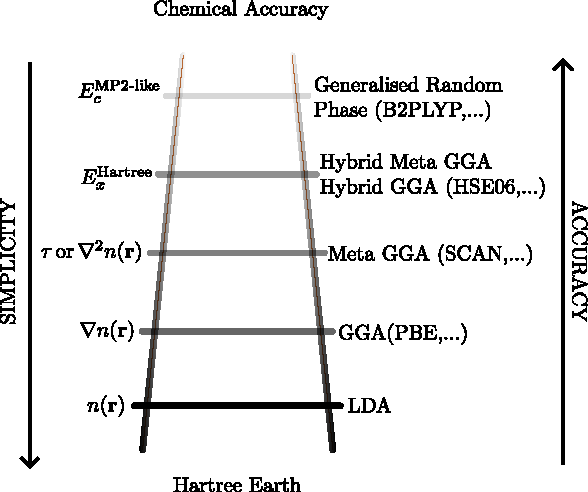
\includegraphics[width=0.6\textwidth]{Jacob-ladder.pdf}
  \caption{Jacob's ladder of exchange-correlation functionals as proposed by J. Perdew\supercite{Perdew2001}. The ladder categorises the functionals into rungs, from the simplest approximation (LDA) at the bottom, progressing to more sophisticated and accurate approximations (Generalised Random Phase) at the uppermost rung.  
  }
  \label{fig:jacob-ladder}
\end{figure}

%\section{Density Functional Tight Binding}
%This is a placeholder 

\section{Ab initio Molecular Dynamics} 
Molecular dynamics (MD)\supercite{marx2009ab, Kuhne2014} is a widely used computational method, which allows us to simulate a many-body condensed matter system and to compute its thermodynamic and dynamical properties. In MD, a system is modelled as a collection of particles---atoms or molecules--- whose trajectories evolve under the influence of interatomic forces following Newton's equations of motion. 


One of the most challenging, yet crucial, aspects of MD is the calculation of the interatomic forces. In classical MD, these forces are typically computed using predefined potential functions or force fields, either constructed upon empirical data or from independent electronic structure calculations that have been parameterised to reproduce experimental or \emph{ab initio} data for small reference systems. Despite their fair success---which we acknowledge but shall not discuss in detail---these empirical interatomic potentials are often limited in their accuracy and transferability. Certain atoms, molecules, or even large systems may give rise to extremely complex interatomic interactions that, if attempted to be modelled with empirical potentials, would demand a rather significant amount of effort. Likewise, these potentials are very often limited to a narrow range of configurations, making them ill-suited for processes involving significant structural changes, such as phase transitions or large deformations.  

Therewith, classical MD can be extended by a first-principles approach, where the interatomic forces are computed on-the-fly from accurate electronic structure calculations, ultimately leading to \emph{ab initio} molecular dynamics (AIMD). This approach allows us to overcome the outlined limitations of classical MD, albeit at a significant computational cost. AIMD employs electronic structure methods such as DFT to compute the interatomic forces at each time step, without relying on predefined interatomic potentials, providing AIMD with an improved predictive power and flexibility.  


\subsection{Hellmann-Feynman Theorem}
 The Hellmann-Feynman theorem\supercite{Feynman1939, Politzer2018} stablishes a relation between the derivative of the total energy $E$ of a system with respect to a parameter $\lambda$ and the expectation value of the derivative of the Hamiltonian with respect to that same parameter.
 While the proof of this theorem is rather straightforward---as shown later in this section---
 it plays a pivotal role in computing interatomic forces in AIMD. 
 
To this end, let us consider the total energy of a system 
\begin{equation}
	\label{69}
	E = \langle \Psi \big| \hat{H} \big| \Psi \rangle
\end{equation}
If $\lambda$ is a parameter that appears explicitly in the Hamiltonian, then 
\begin{equation}
	\label{eq70}
\begin{aligned}
	\frac{\partial E}{\partial \lambda} &= \frac{\partial}{\partial \lambda} \langle \Psi \big| \hat{H} \big| \Psi \rangle \\
  &= \bigg\langle \Psi \bigg| \frac{\partial \hat{H}}{\partial \lambda} \bigg| \Psi \bigg\rangle + \bigg\langle \frac{\partial \Psi}{\partial \lambda} \bigg| \hat{H} \bigg| \Psi \bigg\rangle +  \bigg\langle \Psi \bigg| \hat{H} \bigg|  \frac{\partial \Psi}{\partial \lambda}  \bigg\rangle
\end{aligned}
\end{equation}
Provided that $\hat{H}$ is hermitian and $\Psi$ is an eigenstate of the hamiltonian, $\hat{H}|\Psi\rangle = E|\Psi\rangle$,
Equation \ref{eq70} simplifies to
\begin{equation}
    \label{eq71}
    \begin{aligned}
        \frac{\partial E}{\partial \lambda} &= 
    \bigg\langle \Psi \bigg| \frac{\partial \hat{H}}{\partial \lambda} \bigg| \Psi \bigg\rangle + 
    \bigg\langle \frac{\partial \Psi}{\partial \lambda}\bigg| \hat{H} \bigg| \Psi \bigg\rangle +  
    \bigg\langle\frac{\partial \Psi}{\partial \lambda}\bigg|\hat{H}\bigg|\Psi \bigg\rangle \\
    &=\bigg\langle \Psi \bigg| \frac{\partial \hat{H}}{\partial \lambda}
        \bigg| \Psi \bigg\rangle + E\frac{\partial}{\partial \lambda}
        \langle \Psi|\Psi \rangle + E\frac{\partial}{\partial \lambda}
        \langle \Psi|\Psi \rangle \\
    \end{aligned}
\end{equation}
where the last two terms add up to zero, so that Equation \ref{eq71} becomes,
\begin{equation}
    \label{eq72}
    \frac{\partial E}{\partial \lambda} = 
    \bigg\langle \Psi \bigg| \frac{\partial \hat{H}}{\partial \lambda} \bigg| \Psi \bigg\rangle 
\end{equation}
yielding the Hellmann-Feynman theorem. 

When $\lambda$ corresponds to the position of a nucleus, the negative 
derivative of the total energy with respect to $\lambda$ results 
in the force acting on that nucleus.  More 
generally, the force on nucleus $I$ can be expressed as 
the negative gradient of the total energy with respect to its position $R_I$,
\begin{equation}
    \label{eq73}
    \mathbf{F}_I = -\nabla_{R_I} \langle \Psi | \hat{H} | \Psi \rangle
\end{equation}
This result---referred to as the Hellmann-Feynman force---provides a 
fundamental connection between the quantum mechanical energy landscape and the 
classical nuclei motion in AIMD. 
\subsection{Born-Oppenheimer Molecular Dynamics}
As previously discussed, AIMD relies on solving the static electronic structure 
problem at each time step, given a set of fixed nuclear positions at a certain instant in time.
One approach to achieve this is the so-called Born-Oppenheimer molecular dynamics 
(BOMD)\supercite{Kuhne2014}, wherein the potential energy $E[\{\psi_{i}\}; \mathbf{R}]$ 
is minimised at each time step with respect to the single-electron wavefunctions
$\{\psi_{i}(\mathbf{r})\}$ under the orthonormality constraint 
$\langle \psi_i(\mathbf{r}) | \psi_j(\mathbf{r}) \rangle = \delta_{ij}$. 
The result is a potential energy surface on which the nuclei evolve classically.

This leads to the following Lagrangian
\begin{equation}
    \label{eq74}
    \mathcal{L}_{\text{BO}}(\{\psi_{i}\}; \mathbf{R}, \dot{\mathbf{R}}) =
    \frac{1}{2}\sum_{I} M_{I} \dot{\mathbf{R}}_{I}^2 - \min_{\{\psi_{i}\}} E[\{\psi_{i}(\mathbf{r})\}; \mathbf{R}]
    + \sum_{ij} \lambda_{ij} \left( \langle \psi_i | \psi_j \rangle - \delta_{ij} \right)
\end{equation}
where the first term on the right-hand side corresponds to the classical kinetic energy of the nuclei. The second term,
$E[\{\psi_{i}\}; \mathbf{R}] = E^{\text{KS}}[\{\psi_{i}[n(\mathbf{r})]\}; \mathbf{R}] + E_{II}$, is the total potential energy consisting of the Kohn-Sham ground-state energy and the nuclear-nuclear interaction energy.

By applying the Euler-Lagrange equations to Equation \ref{eq74}
\begin{equation}
    \label{eq75}
\begin{aligned}
    \frac{d}{dt}\frac{\partial \mathcal{L}}{\partial \dot{\mathbf{R}}_{I}} =& \frac{\partial \mathcal{L}}{\partial \mathbf{R}_{I}} \\
    \frac{d}{dt}\frac{\partial \mathcal{L}}{\partial \langle\dot{\psi}_{i}|} =& \frac{\partial \mathcal{L}}{\partial \langle\psi_{i}|}
\end{aligned}
\end{equation}
we obtain the equations of motion 
    \begin{align}
        M_{I}\ddot{\mathbf{R}}_{I} &= -\nabla_{\mathbf{R}_{I}} \left[\min_{\{\psi_{i}\}} E[\{\psi_{i}(\mathbf{r})\}; \mathbf{R}]\bigg|_{\{\langle \psi_i(\mathbf{r}) | \psi_j(\mathbf{r}) \rangle = \delta_{ij}\}} \right]\label{eq76} \\
        0 &= -\hat{H}^{\text{KS}}|\psi_{i}\rangle  + \sum_{j} \lambda_{ij} | \psi_j \rangle \label{eq77}
    \end{align}
where Equation \ref{eq76} corresponds to the classical Newtonian equations of motion for the nuclei, and Equation \ref{eq77} represents the Kohn-Sham eigenvalue problem.  

Finally, AIMD simulations may also include temperature control, which can be achieved by coupling a thermostat to the system in order to simulate different thermodynamic ensembles---\emph{e.g.}, canonical (NVT) or isothermal-isobaric (NPT) ensembles.
However, the details of thermostats and different ensembles are beyond the scope of this report, and we shall refer the reader to the literature\supercite{tuckerman2023statistical,frenkel2023understanding} for a more detailed discussion of these topics.

\section{Computational Implementation in VASP}
The computational studies presented in this report were performed using the Vienna Ab initio Simulation Package (VASP). This is a software suited for performing \emph{ab initio} quantum mechanical calculations\supercite{https://doi.org/10.1002/jcc.21057}. It employs DFT as the basic method, albeit it also allows for beyond-DFT methods such as hybrid functionals, many-body perturbation theory (the GW method) and random phase approximation (RPA). 

VASP is widely adopted in areas such as materials science, condensed matter physics and quantum chemistry, owing to its demonstrated accuracy and state-of-the-art methods. Consequently, this section is devoted to explaining some important aspects of VASP, with great emphasis on the computational methods employed in this work. 

\subsection{Pseudopotentials}
An important step towards defining the wavefunctions that describe an atom is the effective modelling of the electron-ion potential. In this context, core electrons represent a challenge since their rapidly oscillating wavefunctions require a denser real-space grid and a larger number of basis functions to be accurately represented.

To circumvent this problem, we first need to consider the fact that core electrons are tightly bound and do not participate in chemical bonding. Therefore, we can treat them as frozen---\emph{i.e.}, keeping them in their ground state and isolated from the solid-state environment---focusing the calculations on valence electrons, as they do participate in chemical bonding and determine the material's properties. Nonetheless, any adopted approximation must adequately account for the influence of core electrons on the valence states, such as screening and exchange interactions.

To this end, we shall introduce the concept of pseudopotentials\supercite{Hellmann1935}. This approximation aims to describe the valence electrons without explicitly treating the core states, replacing the strong Coulomb potential near the nucleus with a weaker one. We start by splitting the single-electron states into valence and core states, identified as $|\psi_{v}\rangle$ and $|\psi_{c}\rangle$, respectively. We then define a new set of valence states $|\tilde{\psi}_{v}\rangle$  through the following relation 
\begin{equation}
    \label{eq78}
    |\tilde{\psi}_{v}\rangle = |\psi_{v}\rangle + \sum_{c} |\psi_{c}\rangle 
    \langle \psi_{c} |\tilde{\psi}_{v}\rangle
\end{equation}
Applying the single-particle Hamiltonian $H^{sp}$ to the pseudo-valence states, and taking into account that $|\psi_{v}\rangle$ and $|\psi_{c}\rangle$ are eigenstates of the single-particle Hamiltonian, we get
\begin{equation}
    \label{eq79}
    \begin{aligned}
    H^{sp} |\tilde{\psi}_{v}\rangle &= H^{sp}|\psi_{v}\rangle  + 
    \sum_{c} H^{sp}|\psi_{c}\rangle \langle \psi_{c} |\tilde{\psi}_{v}\rangle\\
    &= \epsilon_{v} |\psi_{v}\rangle + \sum_{c} \epsilon_{c} |\psi_{c}\rangle
    \langle \psi_{c} |\tilde{\psi}_{v}\rangle\\
    &= \epsilon_{v} |\psi_{v}\rangle + \sum_{c} (\epsilon_{c} - \epsilon_{v}) |\psi_{c}\rangle
    \langle \psi_{c} |\tilde{\psi}_{v}\rangle\\
    \end{aligned}
\end{equation}
Rearranging the terms, we obtain the following expression
\begin{equation}
    \label{eq80}
    \left[H^{sp} + \sum_{c} (\epsilon_{v} - \epsilon_{c})|\psi_{c}\rangle \langle \psi_{c} | \right] 
    |\tilde{\psi}_{v}\rangle = \epsilon_{v} |\tilde{\psi}_{v}\rangle
\end{equation}
Equation \ref{eq80} describes the Hamiltonian of the pseudo-valence states, which we can define as 
\begin{equation}
    \label{eq81}
    \hat{H}^{ps} = H^{sp} + \sum_{c} (\epsilon_{v} - \epsilon_{c})|\psi_{c}\rangle \langle \psi_{c} |
\end{equation}
The modified potential for these states is called the pseudopotential, given by 
\begin{equation}
    \label{eq82}
    V^{ps}(\mathbf{r}) = V^{sp} + \sum_{c} (\epsilon_{v} - \epsilon_{c})|\psi_{c}\rangle \langle \psi_{c} |
\end{equation}
We emphasise that the pseudo-valence states associated with Equation \ref{eq80} has the same single-particle energies as the valence states, and they remain orthogonal to the core states. However, they are not strictly normalised, which can introduce minor inaccuracies in practical calculations. 

Various pseudopotentials have been proposed to achieve the desired trade-off between accuracy and computational cost. Those pseudopotentials requiring larger cut-off energies---hard pseudopotentials---are better suited for capturing the strong interactions inherent in core electrons. In contrast, soft pseudopotentials are often preferred as they require fewer basis functions, reducing the computational cost, albeit at the expense of accuracy.

\subsection{Projector Augmented-Wave (PAW) Method in VASP}
The projector augmented wave (PAW) method---implemented in VASP and used in this work---aims to address some limitations of pseudopotentials by introducing auxiliary functions called projectors, allowing for core and valence electrons to be better represented and enhance computational efficiency. 

However, before we introduce the PAW formalism---at least to the extent necessary for this report---we shall first introduce some important concepts that underpin the PAW method.
\subsubsection{Key Concepts}
\begin{itemize}
    \item \textbf{Brillouin Zone and k-points}

    Crystalline solids are described in real space in terms of a primitive unit cell (PUC)\supercite{kaxiras2003atomic}, which is the smallest repeating unit capable of generating the entire solid through periodic boundary conditions. It is characterised by a periodic arrangement of lattice points, referred to as the Bravais lattice. All the lattice points are associated with a set of lattice vectors $\mathbf{R}$ formed by all the possible combinations of integer multiples of the primitive lattice vectors 
    $\mathbf{a}_1$, $\mathbf{a}_2$ and $\mathbf{a}_3$

    \begin{equation}
        \label{eq83}
        \mathbf{R} = n_1\mathbf{a}_1 + n_2\mathbf{a}_2 + n_3\mathbf{a}_3, \quad n_1, n_2, n_3 \in \mathbb{Z}
    \end{equation}
    The primitive unit cell is then defined as the volume enclosed by the primitive lattice vectors 
    \begin{equation}
        \label{eq84}
        V_{PUC} = \mathbf{a}_1 \cdot (\mathbf{a}_2 \times \mathbf{a}_3)
    \end{equation}
Using this definition, it is possible to represent the entire crystal by
modelling solely its unit cell. Additionally, to appropriately describe 
electronic properties, we must transition to reciprocal space, defined by
the reciprocal vectors 
\begin{equation}
    \label{eq85}
    \mathbf{b}_1 = \frac{2\pi}{V_{PUC}} (\mathbf{a}_2 \times \mathbf{a}_3), \quad
    \mathbf{b}_2 = \frac{2\pi}{V_{PUC}} (\mathbf{a}_3 \times \mathbf{a}_1), \quad
    \mathbf{b}_3 = \frac{2\pi}{V_{PUC}} (\mathbf{a}_1 \times \mathbf{a}_2)
\end{equation}
that satisfy the condition $\mathbf{a}_{i}\vdot \mathbf{b}_{j} = 2\pi \delta_{ij}$. Any 
reciprocal lattice vector $\mathbf{G}$ can then be expressed as
\begin{equation}
    \label{eq86}
    \mathbf{G} = m_1\mathbf{b}_1 + m_2\mathbf{b}_2 + m_3\mathbf{b}_3, \quad m_1, m_2, m_3 \in \mathbb{Z}
\end{equation}

The reciprocal space is divided into regions called Brillouin zones (BZs). The first Brillouin zone is defined as the region in reciprocal space closest to the origin ($\Gamma$ point). Moreover, the volume of the first BZ is given by
\begin{equation}
    \label{eq87}
    V_{BZ} = \frac{(2\pi)^3}{V_{PUC}}
\end{equation}
which ensures consistency between the real and reciprocal spaces, and proper normalisation when integrating physical quantities over the BZ.

Finally, because electrons in a crystal are subjected to a periodic potential, single-electron wavefunctions follow Bloch's theorem and can be expressed as 
\begin{equation}
    \label{eq88}
    \psi_{\mathbf{k}} = e^{i\mathbf{k} \cdot \mathbf{r}} u_{\mathbf{k}}(\mathbf{r})
\end{equation}
where $\mathbf{k}$ is the wave vector inside the first BZ, and 
$u_{\mathbf{k}}(\mathbf{r}) = u_{\mathbf{k}}(\mathbf{r}+\mathbf{R})$ is a periodic function of the Bravais lattice.
Many quantities---such as the total energy, electronic density and the total density of states---
can be computed by integrating functions of $\mathbf{k}$ over the 
Brillouin zone, 
\begin{equation}
    \label{eq89}
    \langle A \rangle = \frac{V_{PUC}}{(2\pi)^3} \int_{BZ} A(\mathbf{k}) d\mathbf{k}
\end{equation}
Attempting to compute this integral over the entire BZ would require an infinite number of $\mathbf{k}$ points, which is intractable in practice. Instead, we can discretise the BZ into a finite number of $\mathbf{k}$ points. In VASP, it is achieved by following the Monkhorst-Pack\supercite{Monkhorst1976} scheme, 
\begin{equation}
    \label{eq90}
    \mathbf{k} = \sum_{i=3}^{3} \frac{n_i + s_i + \frac{1 - N_i}{2}}{N_1} \mathbf{b}_i 
\end{equation}
where $n_i$ are indices representing the subdivisions along each reciprocal lattice vector, $s_i$ is an optional shift in terms of subdivisions, and $N_i$ is the total number of subdivisions along the $\mathbf{b}_i$ direction. 
 
Ultimately, the Monkhorst-Pack scheme allows us to generate a uniform and symmetrical grid of $\mathbf{k}$ points in the BZ, and, consequently, to compute integrals over the BZ by summing over a finite number of $\mathbf{k}$ points. 

    \item \textbf{Plane-Wave Expansion and Cut-off Energy}  
    
Following from our previous discussion---where we expressed the single-electron wavefunction as a combination of a periodic function and a plane wave---we can expand $u_{\mathbf{k}}(\mathbf{r})$ in terms of a set of plane waves 
\begin{equation}
\label{eq91}
    u_{\mathbf{k}}(\mathbf{r}) = \sum_{\mathbf{G}} C_{\mathbf{G}} e^{i\mathbf{G} \cdot \mathbf{r}}
\end{equation}

Combining Equations \ref{eq88} and \ref{eq91}, gives 
\begin{equation}
    \label{eq92}
    \psi_{\mathbf{k}}(\mathbf{r}) =
    \sum_{\mathbf{G}} C_{\mathbf{k+G}} e^{i(\mathbf{k} + \mathbf{G}) \cdot \mathbf{r}}
\end{equation}
where $C_{\mathbf{k+G}}$ are the corresponding Fourier coefficients 
associated to the plane wave of wavevector $\mathbf{k} + \mathbf{G}$.

Noticeably, Equation \ref{eq92} introduces a new complexity in the calculations---the evaluation of a single k-point requires the summation over an infinite number of possible $\mathbf{G}$ vectors. However, the interpretation of Equation \ref{eq92} as solutions to the Schrödinger equation allows for the kinetic energy to be expressed as
\begin{equation}
    \label{eq93}
    E_{\text{kin}} = \frac{1}{2} |\mathbf{k} + \mathbf{G}|^2
\end{equation}
In practice, lower energy solutions are more physically relevant, thereby allowing us to truncate the infinite summation by including only plane waves whose kinetic energy does not exceed a certain cut-off energy
$E_{\text{cut}}$
\begin{equation}
\label{eq94} 
\frac{1}{2} |\mathbf{k} + \mathbf{G}|^2 \leq E_{\text{cut}}
\end{equation}
This gives a finite expansion
\begin{equation}
    \label{eq95}
    \psi_{\mathbf{k}}(\mathbf{r}) = \sum_{|\mathbf{k} + \mathbf{G}|^2/2 \leq E_{\text{cut}}}
C_{\mathbf{k}+\mathbf{G}} \, e^{i(\mathbf{k} + \mathbf{G}) \cdot \mathbf{r}}
\end{equation}
Finally, in VASP, we often set the cut-off energy based on a convergence criterion of the total energy of the system 
\begin{equation}
\label{eq96}
    \Delta E_{tot} < 1 \text{meV/atom}
\end{equation}
ensuring a good description of the electronic structure of the system and keeping the calculations computationally feasible.

\end{itemize}

\subsubsection{Projector Augmented-Wave (PAW) Method}
Having explored the base concepts of the Projector Augmented-Wave (PAW) method---regarding its implementation in VASP---we can transition to the PAW formalism itself. The PAW method was first introduced by P. E. Bl\"ochl\supercite{Blochl1994} as a generalisation of the pseudopotential method and linear augmented plane-wave method. Later on, it was further refined by G. Kresse and J. Joubert\supercite{Kresse1999} providing a formal relationship between ultra-soft pseudopotentials and the PAW method. 

The PAW method addresses the problem of describing the valence states with high accuracy while accounting for the large variations in the all-electron (AE) wavefunction near the atomic core. It does so by introducing a transformation that maps pseudo (PS) wavefunctions---smooth and computationally efficient---onto their corresponding AE counterparts. Thereby, any AE Kohn-Sham wavefunction $\Psi_n$ can be recovered from a PS wavefunction $\tilde{\Psi}_n$ by means of a linear tranformation
\begin{equation}
    \label{eq97}
    \ket{\Psi_n} = |\tilde{\Psi}_n\rangle + \sum_{i} \left( 
        \ket{\phi_i} - |\tilde{\phi}_i\rangle \right)
        \langle \tilde{p}_i | \tilde{\Psi}_n \rangle
\end{equation}
where important elements are to be highlighted:
\begin{itemize}
    \item AE partial wavefunctions $\ket{\phi_i}$, obtained from a reference atom. 
    \item PS partial wavefunctions $|\tilde{\phi}_i\rangle$, which match the AE wavefunctions outside a core radius $r_c$
    \item Projector functions $\ket{\tilde{p}_i}$, which quantify the contribution of the difference $\ket{\phi_i} - |\tilde{\phi}_i\rangle$ to be added to the PS wavefunction in order to recover the AE wavefunction. They fulfil the biorthonormality condition $\langle \tilde{p}_i | \tilde{\phi}_j \rangle = \delta_{ij}$ within the augmented region, ultimately leading to the completeness relation $\sum_i |\tilde{\phi}_i\rangle \langle \tilde{p}_i| = \mathbb{1}$ .
\end{itemize}
Additionally, in the PAW method, the total AE electronic density is expressed as 
\begin{equation}
    \label{eq98}
    n(\mathbf{r}) = \tilde{n}(\mathbf{r}) + n^1(\mathbf{r}) - \tilde{n}^1(\mathbf{r})
\end{equation}
where $\tilde{n}$ is the PS valence electronic density, $n^1$ is the AE one-center electronic density accounting for the contribution of the valence states inside the augmentation region, and $\tilde{n}^1$ is the corresponding PS one-center electronic density.

Finally, the PAW method helps us to recover the true AE electronic density by correcting the PS electronic density within the augmentation region. As a result, many electronic structure properties---such as the total energy, forces and stresses---can be accurately evaluated.

\subsection{Equation of State (EOS)}
In order to study the mechanical properties of bulk materials, it is important to establish a relationship between observables---such as the ground state total energy---and macroscopic variables like volume or pressure. In this context, the third-order Birch-Murnaghan equation of state\supercite{Birch1947,poirier2000introduction} provides a means to relate the total energy to the change in volume in the system. By fitting energy-volume data to this equation, one can obtain important elastic properties, including equilibrium volume and energy, the bulk modulus and its pressure derivative. This equation is given by 
\begin{equation}
    \label{eq99}
     E(V) = E_0 + \frac{9}{16} V_0 B_0 \left\{ \left[ \left( \frac{V_0}{V} \right)^{2/3} 
     - 1 \right]^3 B_0' + \left[ \left( \frac{V_0}{V} \right)^{2/3} - 1 \right]^2 \left[6 - 4 \left( \frac{V_0}{V} \right)^{2/3} \right] \right\}
\end{equation}
where $E_0$, $V_0$, $B_0$ and $B_0'$ are the equilibrium energy, volume, bulk modulus and its pressure derivative, respectively.

Equation \ref{eq99} is utilised in this work to report the aforementioned thermodynamic properties, which are essential for understanding the material's mechanical response under compression or expansion. 

\subsection{Machine Learning Force Fields (MLFFs)}
In an earlier discussion, we introduced the concept of \emph{ab initio} molecular dynamics (AIMD) and highlighted its importance for determining the dynamical properties of a material. Nonetheless---even though VASP is highly optimised for these calculations---AIMD methods remain computationally expensive, restricting its applicability to small simulation cells and short simulation times. 

In this regard, machine learning force fields (MLFFs) represent a promising alternative. These models are trained on accurate \emph{ab initio} datasets, allowing them to learn the underlying potential energy, thereby producing fast and accurate predictions of atomic energies, forces and stresses. MLFFs can drastically reduce computational cost while minimising any human intervention and expertise required for the force field construction.

In VASP, MLFFs are implemented following an on-the-fly machine learning algorithm\supercite{Jinnouchi2019} (see Figure \ref{fig:MLFF-pipeline}). To construct the machine-learning force field several structure datasets are required. A structure dataset must define the Bravais lattice, atomic positions, total energy, forces and the stress tensor computed from first principles (FP). Given the datasets, local configurations around an atom are identified and mapped onto a set of descriptors\supercite{Jinnouchi2020}, describing the local environment around each atom in terms of an atomic distribution function.

\begin{figure}[H]
    \centering
    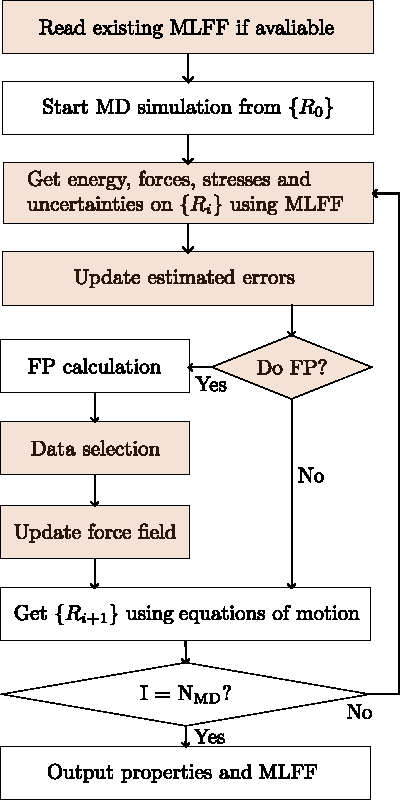
\includegraphics[width=0.4\textwidth]{MLFF-pipeline.pdf}
    \caption{On-the-fly force field generation pipeline in VASP\supercite{Jinnouchi2019}. First, the algorithm reads the existing MLFF if available; otherwise it generates a new one. If accurate enough, a new structure is generated using the force field; otherwise, a first principles calculation is performed. If the predicted uncertainty is too large, the new structure is added to the dataset, and the force field is retrained. This oscillating process between training and prediction continues until we reach the total number of ionic steps specified in the setup.}
    \label{fig:MLFF-pipeline}
\end{figure}
\begin{align}
    \rho_{i}^{(2)}(r) &= \frac{1}{4\pi} \int \rho(r\hat{\mathbf{r}}) d\hat{\mathbf{r}} \label{eq100} \\
    \rho_{i}^{(3)}(r, s, \theta) &= \iint d\hat{\mathbf{r}} d\hat{\mathbf{s}} 
    \, \delta (\hat{\mathbf{r}} \vdot \hat{\mathbf{s}}-\cos{\theta})
    \sum_{j\neq 1}^{\text{N}_{a}}\sum_{k\neq i,j}^{\text{N}_{a}}
    \tilde{\rho}_{ij}(r\hat{\mathbf{r}})\tilde{\rho}_{ik}(s\hat{\mathbf{s}}) \label{eq101}
\end{align}
Equation \ref{eq100} defines the two-body descriptor as the probability of fiding an atom $j(j\neq i)$ at a distance $r$ from atom $i$. Conversely, Equation \ref{eq101} is known as the three-body descriptor and describes the probability to find an atom $j(j\neq i)$ at a distance $r$ from atom $i$ and another atom $k(k\neq i,j)$ at a distance $s$ from atom $i$ spanning an angle $\angle kij$ between them. These descriptors are then used to construct the local potential energy functionals $U_{i}=F[\rho_{i}^{(2)}, \rho_{i}^{(3)}]$ upon which the force field is constructed. 

The force field is then generated during AIMD simulations following the steps below:
\begin{enumerate}
    \item The machine predicts the energy, forces, stress tensor and uncertainty for the current atomic configuration using the available force field. 

    \item The algorithm decided whether to perform an FP calculation or not. This decision is based on the uncertainty of the prediction. If the uncertainty is larger than a predefined threshold, the machine continues to step 3; otherwise, it proceeds to step 5. 

    \item The FP calculation is performed for the current structure, and the obtained dataset is then stored as a candidate for the training dataset. 

    \item If the number of candidate structures reaches a certain threshold, or if the uncertainty becomes too large, the algorithm updates the training set and generates a new force field. 

    \item Update the atomic positons and velocities. If the force field is not accurate enough, the FP energy, forces and stress tensor are used. Otherwise, those predicted by the force field are used. Afterwards, the algorithm returns to step 1 until the total number of ionic steps is reached.
\end{enumerate}

Ultimately, MLFFs provide a powerful and efficient method for performing MD simulations. It combines the accuracy of AIMD with the speed of classical MD, allowing for large and complex condensed matter systems to be studied with remarkable accuracy and efficiency.

\section{Density Functional Tight Binding (DFTB+)}
Density Functional Tight Binding (DFTB) implemented in the DFTB+ code\supercite{Hourahine2020} is a semi-empirical method derived from the Kohn-Sham DFT by performing a Tylor expansion of the total energy functional around a reference electronic density. This method is computationally efficient and allows for simulations involving large systems and large timescales with reasonable accuracy and being much more faster compared to \emph{ab initio} methods. In this work, the GFN1-xTB (Geometry, Frequency, Noncovalent – extended Tight Binding) method was used to perform an initial relaxation previous to the full structure relaxation using VASP.
